\chapter{Analisi del problema \& Progettazione}\label{ch:project}
  Una volta chiariti i requisiti del sistema, il passo successivo riguarda la progettazione dello stesso.
  In particolare, occorre delineare più nel dettaglio l'architettura di massima del sistema, per poi spostare l'attenzione su ciascuna entità interagente.

  % \section{Architettura del sistema}
  Come preventivato già in fase di analisi dei requisiti, il sistema vede la presenza di due principali entità:

  \begin{itemize}
    \item una pagina web che costituisce il client del sistema.
    \item un server di backend, che esegue su piattaforma JVM interfacciandosi con un esecutore di codice Protelis.
  \end{itemize}

  \begin{figure}[htbp]
    \centering
    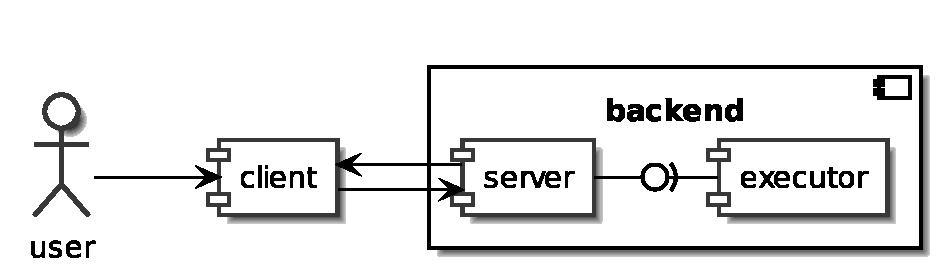
\includegraphics[width=.8\textwidth]{res/uml/architecture-design.eps}%
    \caption{Il diagramma UML riporta l'architettura di massima dei componenti del sistema}%
    \label{fig:architecture-design}
  \end{figure}

  Nelle \nameCrefs{sec:arch:client} successive di questo \nameCref{ch:project}, si intende analizzare più nel dettaglio questa struttura (di cui si ha una rappresentazione grafica in~\Cref{fig:architecture-design}),
  focalizzandosi sui dettagli di ciascun componente.

  \section{Design dell'applicazione}\label{sec:client-design}
    % TODO

    \subsection{Mockup dell'interfaccia}\label{subsec:mockup}
      Una volta chiariti i requisiti e le possibili fonti di ispirazione per la struttura della GUI da realizzare, sono stati disegnati dei mockup che potessero rappresentare una linea guida
      per l'implementazione concreta dell'interfaccia.

      Come detto anche nella~\Cref{subsec:online-ide}, la struttura grafica dell'applicazione dovrebbe ispirarsi a quella di altri ambienti di sviluppo online,
      come ad esempio Overleaf (\Cref{fig:overleaf}).

      \begin{figure}[htbp]
        \centering
        \includegraphics[width=.8\textwidth]{res/fig/overleaf.png}%
        \caption{Screenshot prelevato dalla pagina principale della web app Overleaf}%
        \label{fig:overleaf}
      \end{figure}

      Tali applicazioni hanno generalmente una struttura bipartita:
      nella parte sinistra è solitamente presente un editor che ricorda quello disponibile in diverse IDE desktop, mentre nella parte destra viene generalmente inserita una visualizzazione dell'output.
      Ad esempio, in Overleaf è possibile, alternativamente, visualizzare il log degli errori o il documento compilato.

      \begin{figure}[htbp]
        \centering
        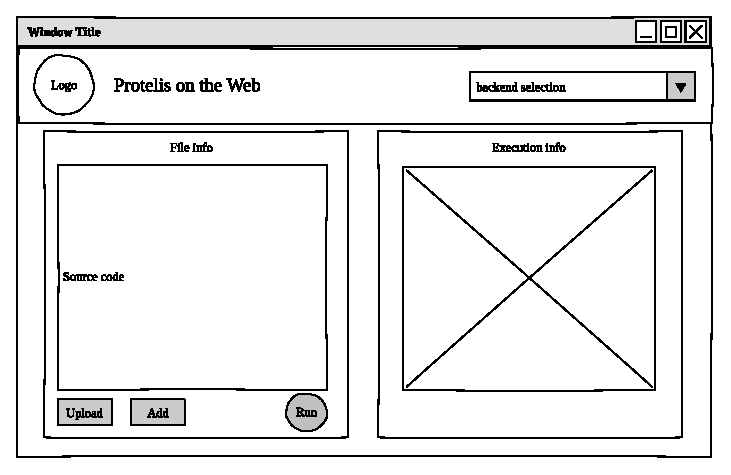
\includegraphics[width=.8\textwidth]{res/mockup/gui-actual.eps}%
        \caption{Mockup dell'interfaccia che dovrà presentare la pagina web}%
        \label{fig:mockup}
      \end{figure}

      Nel mockup finale, riportato in~\Cref{fig:mockup}, si è preso molto ispirazione da questo tipo di struttura.
      L'interfaccia dovrebbe infatti essere costituita dalle seguenti parti:

      \begin{itemize}
        \item
          Una barra superiore, nella quale è riportato il nome e il logo del progetto, insieme a un selettore per il backend.
          Nei primi mockup, tale selettore era posizionato nella sezione principale della pagina, ma successivamente si è preferito spostarlo per sfruttare al meglio lo spazio a disposizione.
        \item
          Un blocco di sinistra, che costituisce la parte con cui l'utente può interagire per lavorare sul codice.
          Il componente principale è appunto l'editor, un campo di testo ``avanzato'' che permette di visualizzare il codice Protelis di esempio e modificarlo.
          Sotto di esso sono presenti i bottoni di controllo per interagire con l'esecuzione.
        \item
          Un blocco di destra, che ospita un canvas in cui l'esecuzione viene rappresentata.
          Al suo interno, verranno visualizzati i nodi su cui il codice sta eseguendo.
          % In questa sezione, i componenti principali sono:
          % \begin{description}
          %   \item[Editor]
          %     Un campo di testo in cui visualizzare codice Protelis di esempio e modificarlo.
          %   \item[Play]
          %     Un bottone che permette di lanciare l'esecuzione del codice.
          %   % \item[Add]
          %   % TODO
          % \end{description}
      \end{itemize}

    \subsection{Design di riferimento}\label{subsec:material}
      Come è stato già sottolineato, l'applicazione vede come utilizzo principale quello dell'utente inesperto del linguaggio.
      L'interfaccia non deve essere solo semplice, ma anche moderna, gradevole e intuitiva.
      Era dunque necessario scegliere uno stile grafico familiare, moderno e facilmente adattabile a quella che sarebbe essere la nuova interfaccia che si stava progettando.

      Prendendo come esempio l'interfaccia di Overleaf (\Cref{fig:overleaf}), è possibile notare come il design di base abbia uno stile di tipo \emph{flat};
      si è deciso dunque di valutare tra i principali design possibili quali fosse più adeguato per la UX che si aveva intenzione di progettare.

      La scelta è infine ricaduta sul Material Design sviluppato da Google:
      dal suo annuncio nel giugno del 2014 al Google I/O 2014 Keynote esso è stato almeno parzialmente adottato in molte applicazioni web, mobile e desktop
      e ben si si presta all'implementazione di un'interfaccia semplice e minimale.

      Per offrire un'esperienza coerente, si è deciso di utilizzare le icone e le direttive in merito a dimensioni e variazioni nella palette di colori fornite da Google\footnote{\url{https://material.io}}.
      Il colore base utilizzato per generare la palette è stato ricavato dall'icona ufficiale di Protelis. % TODO: cite logo

  \section{Architettura del client}\label{sec:arch:client}



  \section{Architettura del server}\label{sec:arch:server}

  \section{Interazioni}
